\documentclass{fh-ium-bama}

% Als nächstes werden einige Zusatzpakete eingebunden; bei Bedarf können weitere
% hinzugefügt werden. Die folgenden Pakete sollten nicht ohne besonderen Grund
% geändert oder entfernt werden:
%
%   inputenc - Erlaubt u.a. die direkte Eingabe von Umlauten im Quelltext.
%   pdffonts - Umschaltung auf Times, Helvetica und Courier/CMTT.
%   babel    - Unterstützung für deutsche und mehrsprachige Texte.
%   graphicx - Standard-Grafikpaket, u.a. zum Einbinden externer Grafiken.

\usepackage[utf8]{inputenc}
%\usepackage[cmtt]{pdffonts}
\usepackage[english,ngerman]{babel}
\usepackage{graphicx}
\usepackage{amsmath}
\usepackage{listings}
\usepackage{cite}
\usepackage{fancyhdr} %%Fancy Kopf- und Fusszeilen
% Babel verwendet als Standard die Sprache, die als letzte angegeben ist. Zur
% besseren Dokumentation kann man sie aber auch nochmal explizit auswählen:
\selectlanguage{ngerman}

% Befehle und Umgebungen, die nicht von LaTeX oder den Zusatzpaketen bereit-
% gestellt werden, lassen sich häufig auf einfache Weise selbst definieren.
% Hier die oft gebrauchte Abkürzung 'z.B.' und eine verbesserte Variante des in
% der Anleitung erwähnten Makros für Matrizen und Vektoren (die unabhängig vom
% pdffonts-Paket funktioniert):

\newcommand{\zb}{z.\,B.{}}
\newcommand{\mat}[1]{{\ensuremath{\mathchoice
  {\mbox{\boldmath$\displaystyle\mathbf{#1}$}}
  {\mbox{\boldmath$\textstyle\mathbf{#1}$}}
  {\mbox{\boldmath$\scriptstyle\mathbf{#1}$}}
  {\mbox{\boldmath$\scriptscriptstyle\mathbf{#1}$}}}}}
\newcommand{\racksorter}{\lstinline|racksorter|}
\newcommand{\stack}{\lstinline|stack|}
\newcommand{\cost}{\lstinline|cost|}
\newcommand{\path}{\lstinline|path|}
\newcommand{\chains}{\lstinline|chains|}
\newcommand{\startIdx}{\lstinline|startIdx|}
\newcommand{\findChains}{\lstinline|findChains|}
\newcommand{\findSPR}{\lstinline|findShortestPathRecursive|}
\newcommand{\findSP}{\lstinline|findShortestPath|}
\newcommand{\None}{\lstinline|None|}
\newcommand{\solcnc}{\lstinline|solutionChainAndCost|}
\newcommand{\dist}{\lstinline|distance|}
\newcommand{\xSize}{\lstinline|xSize|}
\newcommand{\ySize}{\lstinline|ySize|}
\newcommand{\pyads}{\lstinline|pyads|}
% Ausnahmen von der automatischen Silbentrennung werden mit dem Befehl
% \hyphenation definiert und gelten für das ganze Dokument.

\hyphenation{Aktu-ali-sie-rung Screen-shots}
% Code-Listning ---------------------------------------------------------------
\usepackage{color}

\definecolor{mygreen}{rgb}{0,0.6,0}
\definecolor{mygray}{rgb}{0.5,0.5,0.5}
\definecolor{mymauve}{rgb}{0.58,0,0.82}

\definecolor{whiteSmoke}{RGB}{245,245,245}
\definecolor{chocolate}{RGB}{210,105,30}
\definecolor{dodgerblue}{RGB}{28,134,238}
\definecolor{darkseagreen}{RGB}{105,139,105}
\definecolor{darkorange}{RGB}{238,118,0}
\definecolor{myGray}{RGB}{229,229,229}
\lstset{ %   % choose the background color
  breakatwhitespace=false, 
  tabsize=2,
  basicstyle=\ttfamily,               % size of fonts used for the code
  breaklines=true,                      % automatic line breaking only at whitespace
  captionpos=b,                         % sets the caption-position to bottom
  commentstyle=\color{mygreen},         % comment style
  escapeinside={\%*}{*)},               % if you want to add LaTeX within your code
  keywordstyle=\color{black},      % keyword style
  stringstyle=\color{chocolate},        % string literal style
  numbers=none,                         % where to put the line-numbers (none, left, right)
  numbersep=5pt,                        % how far the line-numbers are from the code
  numberstyle=\tiny\color{black},       % the style that is used for the line-numbers
  rulecolor=\color{myGray},         % if not set, the frame-color may be changed on line-breaks within not-black text
  frame=lrtb,
  otherkeywords={printf, fopen_s}
}

% Nach den global gültigen Definitionen beginnt das eigentliche Dokument. Der
% Idee von LaTeX folgend sollten ab hier keine Definition oder Layout-
% Anpassungen mehr vorgenommen werden. Idealer Weise wird jetzt nur noch der
% Inhalt des Dokuments beschrieben; das Layout ist vollständig in der Dokument-
% klasse, den Zusatzpaketen und den eigenen Definitionen festgelegt.

\begin{document}

% Der Befehl \frontmatter passt das Seitenlayout an den Vorspann an. Im  Wesent-
% lichen erfolgt die Nummerierung der Seiten in kleinen römischen Buchstaben.
% Zum Vorspann gehören: Titelseite, Aufgabenbeschreibung, Erklärung zur
% Selbständigkeit, Zusammenfassungen und Verzeichnisse.

\frontmatter

% Die Titelseite wird mit dem Befehl \maketitle erzeugt. Dazu müssen lediglich
% Titel, Autor, Datum, Betreuer und Art der Arbeit angegeben werden. Sollte das
% ausnahmsweise nicht zum gewünschten Ergebnis führen, kann man auch zwischen
% \begin{titlepage} und \end{titlepage} die Titelseite frei gestalten (siehe
% Beispiel in 'titlepage.tex'); es werden dann nur die Kopf- und Fußzeile
% automatisch angelegt. In diesem Fall sollten aber trotzdem die o.g. Angaben
% über die Arbeit vorhanden sein, weil daraus die Meta-Informationen für die
% PDF-Datei und weitere Elemente der Arbeit erzeugt werden. Bei \author und
% \supervisor können mehrere Personen durch \and getrennt werden.

\title{Sortieren eines Hochregallagers in C++ und Python}
\author{Eicke Herbertz \and Dominik Hilbers}
\date{10. Dezember 2017}
\supervisor{Prof. Dr.-Ing. Martin Kohlhase}
\thesistype{Studienarbeit}

%\maketitle

\begin{titlepage}
  \vspace*{20mm}
  \centering
  \large Studienarbeit\\[10mm]
  \textbf{\LARGE Sortieren eines Hochregallagers\\
  in C++ und Python}\\[1ex]
  %Version 1.3\\[10mm]
  von\\[1ex]
  Eicke Herbertz\\
  Dominik Hilbers\\[1ex]
  Mat.-Nr.: 131211 131629\\[45mm]
  \begin{tabular}{ll}
    Prüfer:   & Prof.~Dr.-Ing. Martin Kohlhase\\[1ex]
    Abgabedatum: & 11. Dezember 2017
  \end{tabular}
\end{titlepage}

% Kopf- und FussŸzeilen --------------------------------------------------------- 
\pagestyle{fancy}
\fancyhf{}
%Kopfzeile links bzw. innen
\fancyhead[R]{\thepage} %LE,RO
\fancyhead[C]{} 
%Titel des Dokuments 
\fancyhead[L]{\hyperref[tableofcontents]{Sortieren eines Hochregallagers in C++ und Python}}
%Linie oben
\renewcommand{\headrulewidth}{0.5pt}
%Fusszeile links bzw. innen
\fancyfoot[R]{\today}
\fancyfoot[C]{}
\fancyfoot[L]{Eicke Herbertz und Dominik Hilbers}
%Linie unten
\renewcommand{\footrulewidth}{0.5pt}

% Inhaltsverzeichnis ----------------------------------------------------------
\setcounter{page}{1} 
\tableofcontents
\label{tableofcontents}
%Das erste Kapitel soll auf einer ungeraden Seite beginnen.
\mainmatter

\chapter{Einführung}
Die Automatisierungstechnik bietet die Möglichkeit Hardware in Echtzeit anzusteuern und zu regulieren. Durch TwinCAT3, welches Module zum Simulieren einer SPS auf einem PC-System ermöglicht, können Programme mit bekannten Sprachen wie C, C\#, Python und Ähnlichem entwickelt werden die mit diesen Modulen kommunizieren. So auch im Folgenden, ein Hochregallager wird mit einem in Python entwickelten Programm angesprochen um in kürzester Zeit dieses zu Sortieren.

Zur Durchführung wird auf ein Hochregallager aus Fischertechnik zurückgegriffen, das über Sensoren und Aktuatoren verfügt. Diese werden durch Beckhoffklemmen angesteuert, welche über EtherCAT mit einem Computer verbunden sind.
\begin{center}
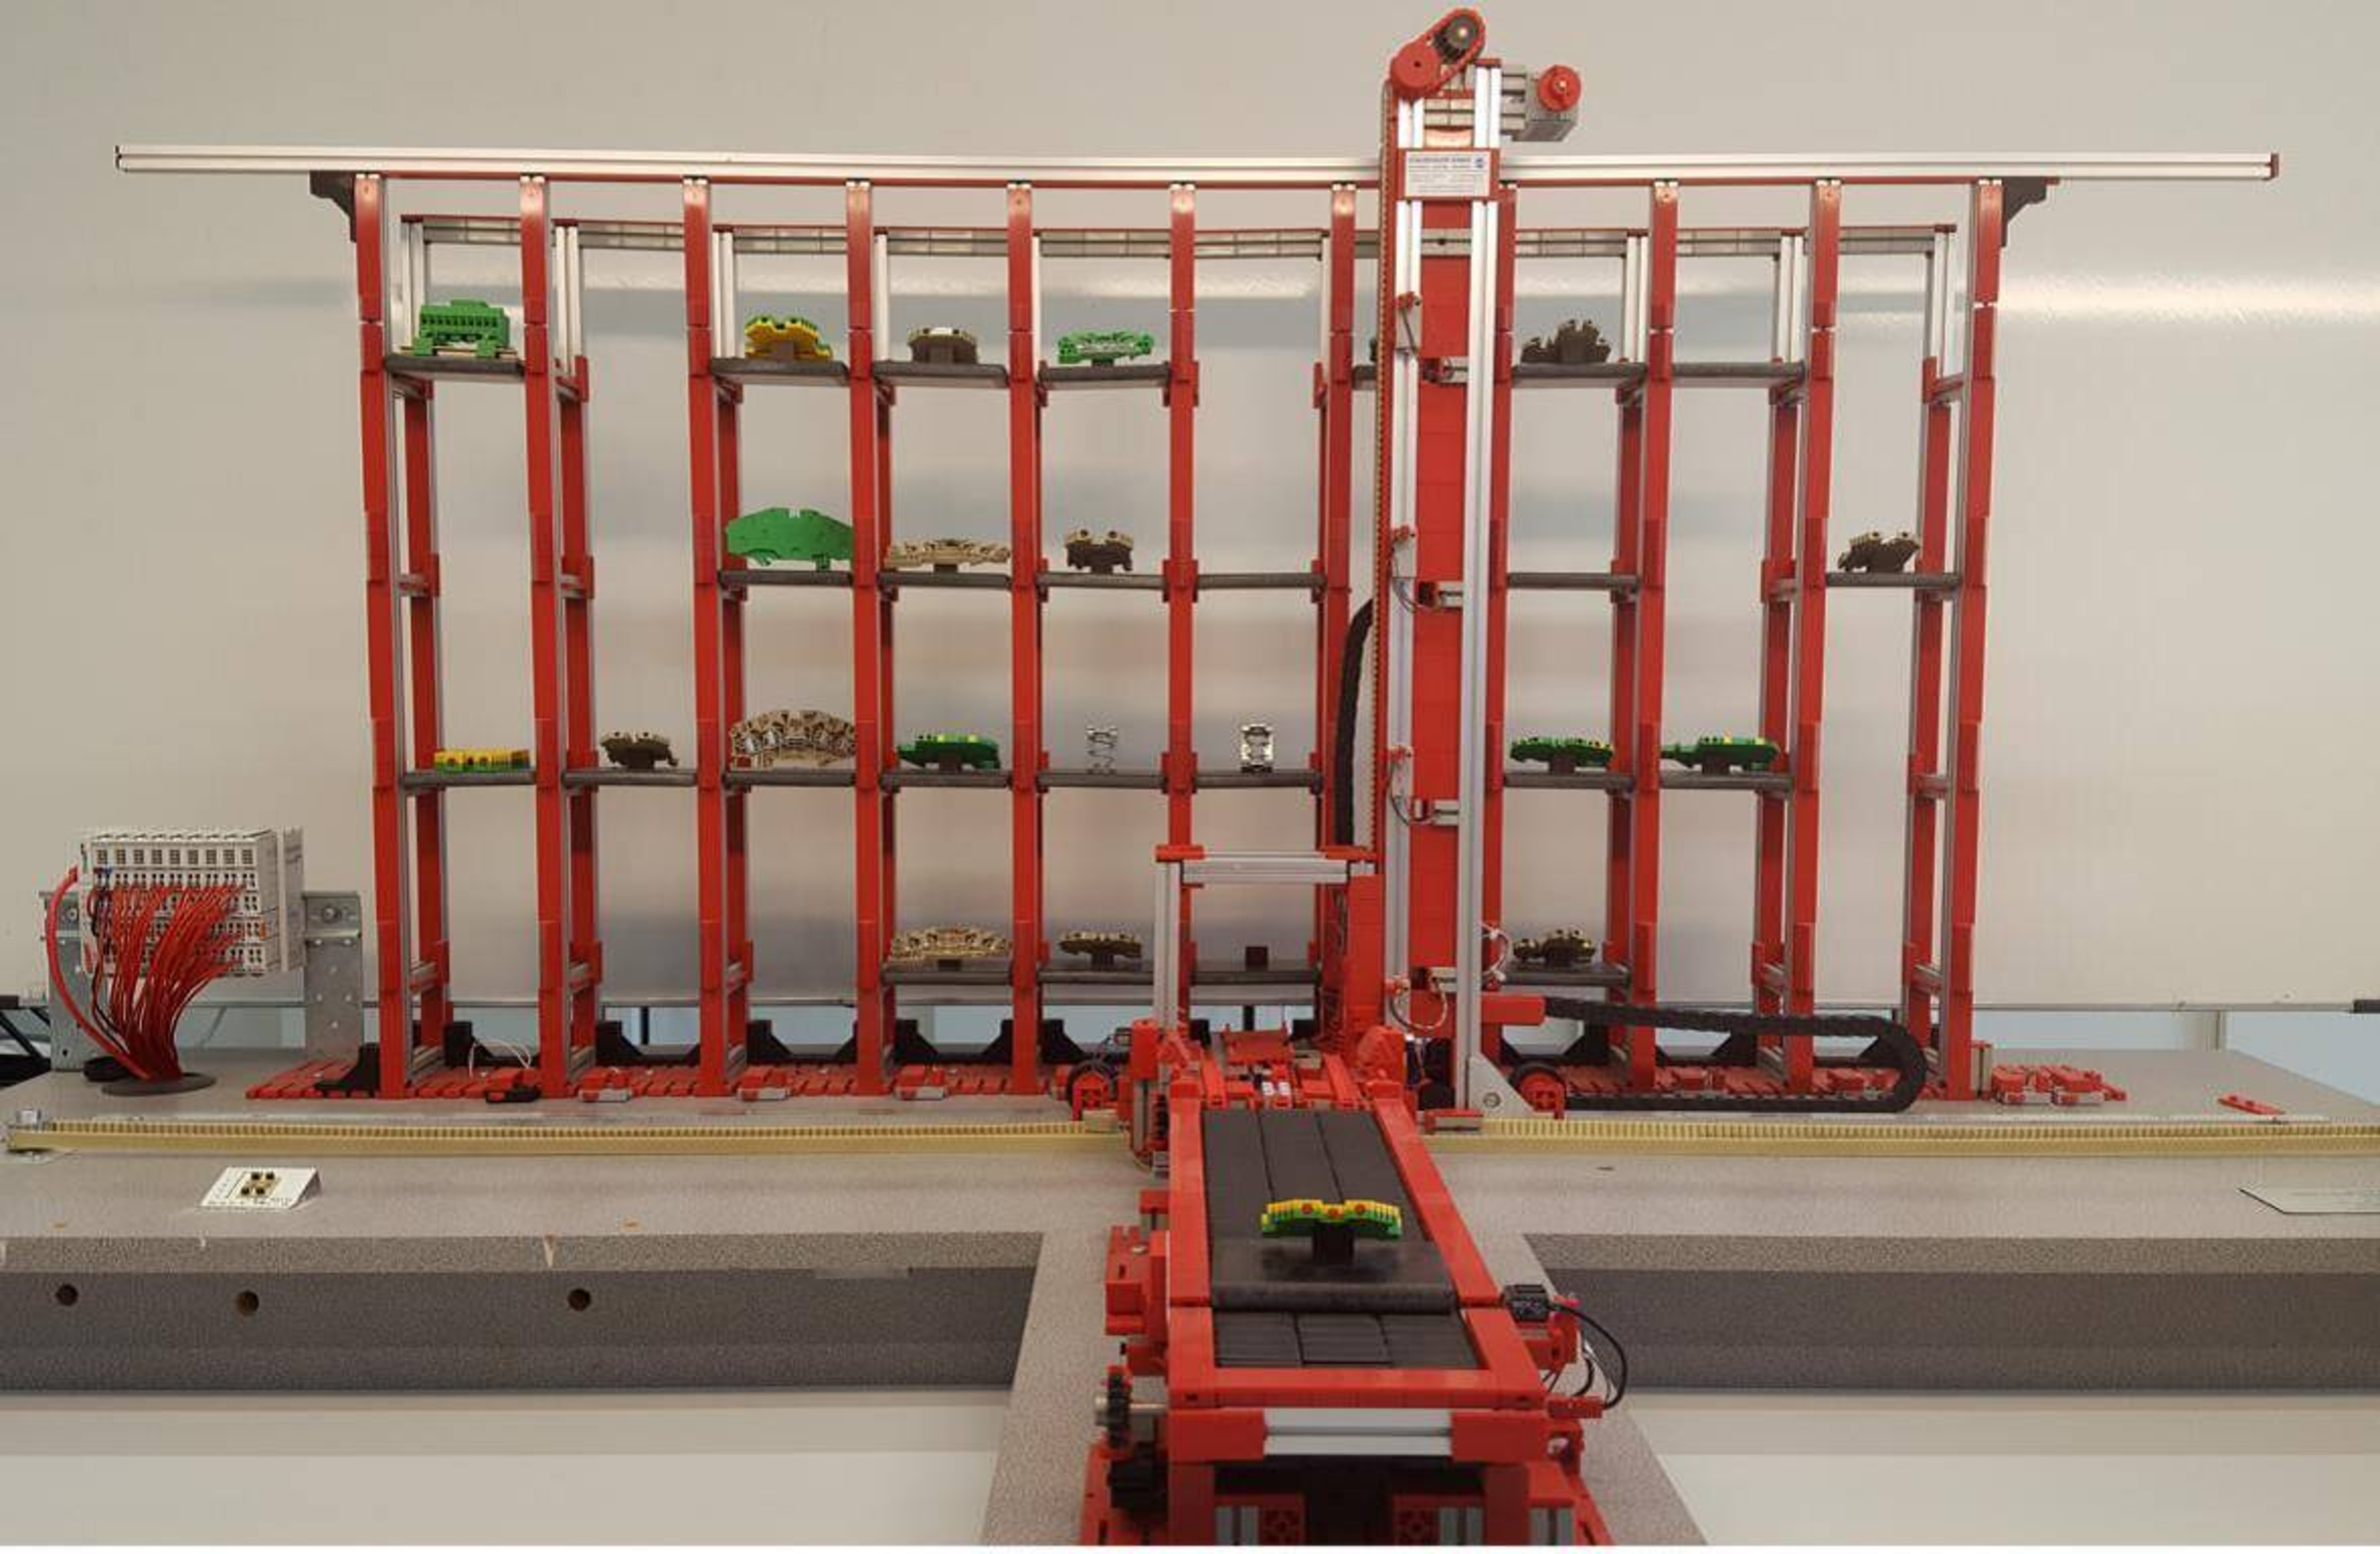
\includegraphics[scale=0.27]{Regal.pdf}
\end{center}
Das Hochregallager hat die Dimension $10x4$ Fächer welche von einem Kran angefahren werden können. Dieser Kran ist mittels Elektromotoren und Riementechnik in x-Richtung bewegbar. An dem Kran ist ein Korb angebracht welcher in y-Richtung agieren kann. Dieser Korb verfügt über einen Schlitten welcher wiederum in z-Richtung fahren kann und die eingelagerten Paletten aufnimmt. An jedem Fach auf Bodenhöhe sind zur x-Positionsermittlung Taster angebracht. Zur Bestimmung der y-Position sind für jede Regalebene zwei Taster mit etwas Abstand zueinander am Kranturm angebracht, diese dienen der Be- und Entladepositionsbestimmung.
Um die Problemstellung vereinfacht darzustellen wird in der Erläuterung von einem 3x3 System ausgegangen und nicht von dem vorhandenen Hochregallager, da dies auf jede beliebige Dimension repliziert werden kann.
\section{Problem}
Gegeben sei ein Lager mit $3$ Spalten und $3$ Reihen, also insgesamt $9$, Lagerplätzen. Acht beliebige dieser Plätze sind mit Elementen belegt und diesen Elementen sind zufällig Wertigkeiten von $1$ bis $8$ zugeordnet. Der leere Platz wird mit einem Unterstrich gekennzeichnet. Ein Beispiel:
\begin{center}
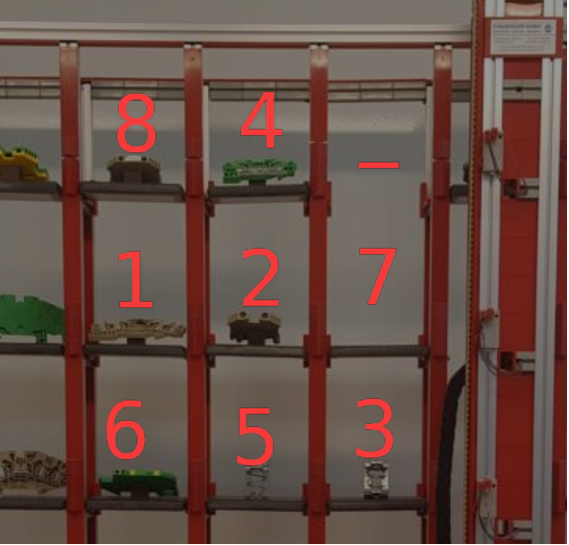
\includegraphics[scale=0.6]{Perm.pdf}
\end{center}
Oder als Matrix:
\begin{gather*}
\begin{bmatrix}
	8 & 4 & \_ \\
	1 & 2 & 7 \\
	6 & 5 & 3
\end{bmatrix}
\end{gather*}
Aufgabe ist, den schnellsten Weg zu finden, um die Elemente in aufsteigender Reihenfolge zu sortieren, mit dem leeren Platz ganz am Ende:
\begin{gather*}
\begin{bmatrix}
	1 & 2 & 3 \\
	4 & 5 & 6 \\
	7 & 8 & \_
\end{bmatrix}
\end{gather*}
Die einzige mögliche Aktion zur Veränderung ist dabei das verschieben eines beliebigen Elements an den aktuell leeren Platz. Hierbei ist zu beachten, dass immer nur ein Element auf einmal entnommen werden kann um dieses zu verschieben.
\newpage
\section{Zielsetzung}
Das Ziel dieses Projektes ist es, ein von einer Beckhoff TwinCAT-Steuerung angesteuertes Hochregallager mit einem leeren Lagerplatz in der schnellstmöglichen Zeit zu sortieren. Hierzu soll ein Modul für TwinCAT3 entwickelt werden und für den Client eine weitere Software Programmiert werden, welche die Auswertung und Berechnung des kürzesten Wegs übernimmt. Auch für die Berechnung des kürzesten Weges muss eine Lösung gefunden werden. Zudem soll ein GUI erstellt werden welche dem Benutzer eine einfache Bedienung ermöglicht.
\newpage
\chapter{Sortieren mit Python}
\section{Permutationen}
{[1]} Um das Problem und den Lösungsweg nachvollziehen zu können, ist es nötig, sich mit Definition und Notation von Permutationen vertraut zu machen. Dazu wird das Problem im Folgenden eindimensional als Mengen betrachtet, die realen Dimensionen finden sich erst in der Kostenfunktion wieder. Die folgende Darstellung wird in den nächsten Abschnitten verwendet:
\begin{gather*}
\begin{bmatrix}
	8 & 4 & \_ \\
	1 & 2 & 7 \\
	6 & 5 & 3
\end{bmatrix}
\Rightarrow
\{8, 4, \_, 1, 2, 7, 6, 5, 3\}
\end{gather*}

\subsection{Definition}
Eine Permutation ist eine bijektive Abbildung $\gamma: X \rightarrow X$ einer Menge $X = \{x_1,x_2,\dots,x_n\}$ mit $n$ Elementen, durch die jedem Element der Menge ein Element der gleichen Menge zugeordnet wird.
Jedes Element $x_i$ für $i = 1,\dots,n$ nimmt bei der Permutation den Platz des ihm zugeordneten Elementes $\gamma(x_i)$ ein.

Im Kontext dieses Problems ist die Zielmenge $X = \{1,2,3,4,5,6,7,8,\_\}$ die Grundlage, allgemein $X = \{1,2,\dots,n-1,\_\}$ für Hochregallager mit $n$ Lagerplätzen.

\subsection{Notation}
\subsubsection*{Zweizeilenform}
In der Zweizeilenform wird die Permutation $\gamma$ als Matrix mit zwei Zeilen und n Spalten dargestellt. Unter jeder Zahl $i = 1,\dots,n$ in der oberen Reihe steht der Funktionswert $\gamma(i)$ in der unteren Reihe:
\begin{gather*}
\gamma =
\begin{pmatrix}
	1 & 2 & \dots & n \\
	\gamma(1) & \gamma(2) & \dots & \gamma(n)
\end{pmatrix}
\end{gather*}
Für die in der Einführung dargestellte Permutation $X_P = \{8, 4, \_, 1, 2, 7, 6, 5, 3\}$ sieht diese Notation so aus:
\begin{gather*}
\gamma_P =
\begin{pmatrix}
	1 & 2 & 3 & 4 & 5 & 6 & 7 & 8 & \_ \\
	4 & 5 & \_ & 2 & 8 & 7 & 6 & 1 & 3
\end{pmatrix}
\end{gather*}
Dabei ist zu beachten, dass die untere Zeile \textit{nicht} direkt der Permutation entspricht. Würde man die Spalten der Matrix nun aber sortiert nach dem Wert der unteren Zeile anordnen, enthielte die obere Zeile die Permutation:
\begin{gather*}
\gamma'_P = 
\begin{pmatrix}
	8 & 4 & \_ & 1 & 2 & 7 & 6 & 5 & 3 \\
	1 & 2 & 3 & 4 & 5 & 6 & 7 & 8 & \_
\end{pmatrix}
\end{gather*}
Diese Darstellung soll nur dem besseren Verständnis dienen und wird so nicht genutzt.

\subsubsection*{Zykelschreibweise}
Für die vorliegende Arbeit ist die Zykelschreibweise allerdings von weitaus höherer Bedeutung als die Zweizeilenform. Um die Permutation auf diese Weise darzustellen, beginnt man mit einer beliebigen Zahl $a \in \{1,\dots,n\}$ und schreibt
\begin{gather*}
(a ~ \gamma(a) ~ \gamma^2(a) ~ \cdots ~ \gamma^{l_a-1}(a))\text{.}
\end{gather*}

Dabei bedeutet $\gamma^k$, dass $\gamma$ $k$ mal hintereinander ausgeführt wird, also $\gamma^2(a) = \gamma(\gamma(a))$. $l_a$ ist die kleine natürliche Zahl mit $\gamma^{l_a}(a) = a$. So hat man einen Zyklus der Permutation beschrieben. Wurden noch nicht alle Zahlen notiert, wählt man aus den übrigen eine Zahl $b$ und verfährt mit ihr genau so.

Für die Permutation $\gamma_P$, zum Beispiel mit $a = 1$, ergibt sich $(1 ~ 4 ~ 2 ~ 5 ~ 8)$. Übrig bleiben $\{3, 6, 7, \_\}$. Daraus wählt man nun zum Beispiel $b = 3$ und erhält $(3 ~ \_)$. Zuletzt wählt man noch $c \in \{6, 7\}$ und erhält $(6 ~ 7)$. Die gesamte Permutation wird durch Auflistung aller Zyklen beschrieben. Die Reihenfolge der Zyklen ist dabei beliebig wählbar und innerhalb eines Zyklus dürfen die Zahlen zyklisch vertauscht werden:
\begin{gather*}
\gamma_P =
(1 ~ 4 ~ 2 ~ 5 ~ 8)(3 ~ \_)(6 ~ 7) =
(2 ~ 5 ~ 8 ~ 1 ~ 4)(\_ ~ 3)(7 ~ 6)
\end{gather*}
Ergeben sich dabei Zyklen, die nur eine Zahl enthalten, können diese weggelassen werden. Es handelt sich dabei um Zahlen, die an ihrer ursprünglichen Position stehen.
\newpage
Jeder Zyklus beschreibt eine zyklische Permutation einer Untermenge der Zahlen der gesamten Permutation. Eine rein zyklische Permutation hat dementsprechend nur einen Zyklus:
\begin{gather*}
\gamma_Z =
\begin{pmatrix}
	1 & 2 & 3 & 4 & 5 & 6 & 7 & 8 & \_ \\
	2 & 3 & 4 & 5 & 6 & 7 & 8 & \_ & 1
\end{pmatrix}
=
(1 ~ 2 ~ 3 ~ 4 ~ 5 ~ 6 ~ 7 ~ 8 ~ \_)
\end{gather*}
Diese Permutation ergibt die Menge $X_Z = \{\_, 1, 2, 3, 4, 5, 6, 7, 8\}$.
Bei einer zyklischen Permutation werden die Elemente einer Menge im Kreis vertauscht. $1$ nimmt hier den Platz von $2$ ein, $2$ den von $3$ und so weiter bis $\_$ den Platz von $1$ einnimmt.
	
\section{Lösungswege}
\subsection{Zyklische Permutationen}
Nun ist das Ziel, die Menge zu sortieren, nur mit dem leeren Feld "$\_$" für Vertauschungen zur Verfügung. Betrachtet man die Menge $X_Z$ und die dazugehörige Permutation $\gamma_z$ als Zyklus, zeigt sich, dass dieser Zyklus gerade die Lösung liefert, um aus der Menge $X_Z$ wieder die Ausgangsmenge $X$ zu machen.
\begin{gather*}
\gamma_Z = (1 ~ 2 ~ 3 ~ 4 ~ 5 ~ 6 ~ 7 ~ 8 ~ \_)\\
X_Z = \{\_, 1, 2, 3, 4, 5, 6, 7, 8\}
\end{gather*}

Dazu "rotiert" man den Zyklus, bis $\_$ an letzter Stelle steht. Nun wählt man das erste Element des Zyklus und legt es an den leeren Platz $\_$. 
Daraus ergibt sich die Menge $X_{Z1} = \{1, \_, 2, 3, 4, 5, 6, 7, 8\}$ mit dem Zyklus $\gamma_{Z1} = (2 ~ 3 ~ 4 ~ 5 ~ 6 ~ 7 ~ 8 ~ \_)$. Der Zyklus $(1)$ kann dabei weggelassen werden, die $1$ ist sozusagen sortiert.
Mathematisch lässt sich das Verschieben des Elements $x$ an einen leeren Platz so beschreiben, dass die Funktionswerte $\gamma(\_)$ und $\gamma(x)$ – also in diesem Fall $\gamma(1)$ – vertauscht werden.
\begin{gather*}
	\gamma_{Z1}(\_) = \gamma_Z(1)\\
	\gamma_{Z1}(1) = \gamma_Z(\_)\\
	\gamma_{Z1} =
	\begin{pmatrix}
		1 & 2 & 3 & 4 & 5 & 6 & 7 & 8 & \_ \\
		1 & 3 & 4 & 5 & 6 & 7 & 8 & \_ & 2
	\end{pmatrix}
\end{gather*}

Jetzt wird mit der $2$ genau so verfahren und man erhält $X_{Z2} = \{1, 2, \_, 3, 4, 5, 6, 7, 8\}$ mit dem Zyklus $\gamma_{Z2} = (3 ~ 4 ~ 5 ~ 6 ~ 7 ~ 8 ~ \_)$. Danach mit der $3$ und so weiter. Wird die $8$ erreicht und an die leere Stelle platziert, hat auch das leere Feld seinen Zielort erreicht und die Menge entspricht wieder der Ausgangsmenge $X$. Dabei wurde jedes Element genau einmal bewegt und hat nach dieser einen Bewegung seinen Zielort erreicht.

Für jede zyklische Permutation ist dies der schnellste Lösungsweg. Jede andere Methode würde erfordern, dass die Elemente nicht sofort an ihren Zielort gebracht würden und demnach mehr als einmal bewegt werden müssten.

\subsection{Andere Permutationen}
Die meisten Permutationen sind keine zyklischen Permutationen. Mithilfe der Zykelschreibweise lassen sich diese allerdings in mehrere zyklische Permutationen aufteilen. Zurück zur ursprünglichen Beispiel-Permutation.
\begin{gather*}
\gamma_P =
\begin{pmatrix}
	1 & 2 & 3 & 4 & 5 & 6 & 7 & 8 & \_ \\
	4 & 5 & \_ & 2 & 8 & 7 & 6 & 1 & 3
\end{pmatrix} =
(1 ~ 4 ~ 2 ~ 5 ~ 8)(3 ~ \_)(6 ~ 7)
\end{gather*}

Jeder der drei Zyklen $(1~4~2~5~8)$, $(3~\_)$ und $(6~7)$ ließe sich nach den oben genannten Regeln in die entsprechende, sortierte Teilmenge von $X$ umwandeln, wenn er ein leeres Feld \_ enthielte. Dieses ist aber selbstverständlich nur ein einem Zyklus enthalten. Verfährt man mit dem Zyklus $(3~\_)$ wie oben, befinden sich die $3$ und das $\_$ zwar an der richtigen Stelle, die anderen Elemente aber nicht.

Das leere Feld muss als in die anderen Zyklen gelangen. Dazu muss nichts weiter gemacht werden, als ein Element aus einem anderen Zyklus auf den leeren Platz zu legen, um die Zyklen zu verbinden. Wählt man zum Beispiel die $1$, ergibt sich $\gamma_{P1}(\_) = \gamma_P(1) = 4, \gamma_{P1}(1) = \gamma_P(\_) = 3$:
\begin{gather*}
\gamma_{P1} = \begin{pmatrix}
	1 & 2 & 3 & 4 & 5 & 6 & 7 & 8 & \_ \\
	3 & 5 & \_ & 2 & 8 & 7 & 6 & 1 & 4
\end{pmatrix} =
(1 ~ 3 ~ \_ ~ 4 ~ 2 ~ 5 ~ 8)(6 ~ 7)
\end{gather*}
Macht man dasselbe nochmal mit der $6$, erhält man:
\begin{gather*}
\gamma_{P2} = \begin{pmatrix}
	1 & 2 & 3 & 4 & 5 & 6 & 7 & 8 & \_ \\
	3 & 5 & \_ & 2 & 8 & 4 & 6 & 1 & 7
\end{pmatrix} =
(1 ~ 3 ~ \_ ~ 7 ~ 6 ~ 4 ~ 2 ~ 5 ~ 8) 
\end{gather*}
Richtig rotiert ist $(7 ~ 6 ~ 4 ~ 2 ~ 5 ~ 8 ~ 1 ~ 3 ~ \_)$ dann der Lösungsweg für diese Permutation $\gamma_{P2}$. Hinzu kommen die vorangegangenen Bewegungen der $3$ und der $6$ und man erhält einen Lösungsweg für $\gamma_P$: $L_P = [3, 6, 7, 6, 4, 2, 5, 8, 1, 3, \_]$. Diese Liste ist kein Zyklus. Für jedes Element der Liste wird dieses Element von seiner aktuellen Position an die leere Position bewegt, dann wird das nächste Element betrachtet.

Eine andere Lösung würde sich ergeben, wenn man zuerst die $6$ bewegt und dann die $5$:
\begin{gather*}
\gamma_{P1}(\_) = \gamma_P(6) = 7, \gamma_{P1}(6) = \gamma_P(\_) = 3\\
\gamma_{P1} = \begin{pmatrix}
	1 & 2 & 3 & 4 & 5 & 6 & 7 & 8 & \_ \\
	4 & 5 & \_ & 2 & 8 & 3 & 6 & 1 & 7
\end{pmatrix} =
(1 ~ 4 ~ 2 ~ 5 ~ 8)(3 ~ \_ ~ 7 ~ 6)\\
\gamma_{P2}(\_) = \gamma_{P1}(5) = 8, \gamma_{P2}(5) = \gamma_{P1}(\_) = 7\\
\gamma_{P2} = \begin{pmatrix}
	1 & 2 & 3 & 4 & 5 & 6 & 7 & 8 & \_ \\
	4 & 5 & \_ & 2 & 7 & 3 & 6 & 1 & 8
\end{pmatrix} =
(8 ~ 1 ~ 4 ~ 2 ~ 5 ~ 7 ~ 6 ~ 3 ~ \_)\\
L_P = [6, 5, 8, 1, 4, 2, 5, 7, 6, 3, \_]
\end{gather*}

Außerdem besteht zu jedem Zeitpunkt die Möglichkeit, nicht zwei Zyklen zu verbinden, sondern stattdessen ein Element an den richtigen Platz zu bringen. So könnte man zum Beispiel beim gerade erreichten $\gamma_{P1} = (1~4~2~5~8)(7~6~3~\_)$ auch zuerst die $7$ an ihren Platz bringen und dann die beiden Zyklen verbinden:
\begin{gather*}
\gamma_{P1}(\_) = \gamma_P(6) = 7, \gamma_{P1}(6) = \gamma_P(\_) = 3\\
\gamma_{P1} = \begin{pmatrix}
	1 & 2 & 3 & 4 & 5 & 6 & 7 & 8 & \_ \\
	4 & 5 & \_ & 2 & 8 & 3 & 6 & 1 & 7
\end{pmatrix} =
(1 ~ 4 ~ 2 ~ 5 ~ 8)(7 ~ 6 ~ 3 ~ \_)\\
\gamma_{P2}(\_) = \gamma_{P1}(7) = 6, \gamma_{P2}(7) = \gamma_{P1}(\_) = 7\\
\gamma_{P2} = \begin{pmatrix}
	1 & 2 & 3 & 4 & 5 & 6 & 7 & 8 & \_ \\
	4 & 5 & \_ & 2 & 8 & 3 & 7 & 1 & 6
\end{pmatrix} =
(1 ~ 4 ~ 2 ~ 5 ~ 8)(6 ~ 3 ~ \_)\\
\gamma_{P3}(\_) = \gamma_{P2}(5) = 8, \gamma_{P2}(5) = \gamma_{P1}(\_) = 6\\
\gamma_{P3} = \begin{pmatrix}
	1 & 2 & 3 & 4 & 5 & 6 & 7 & 8 & \_ \\
	4 & 5 & \_ & 2 & 6 & 3 & 7 & 1 & 8
\end{pmatrix} =
(8 ~ 1 ~ 4 ~ 2 ~ 5 ~ 6 ~ 3 ~ \_)\\
L_P = [6, 7, 5, 8, 1, 4, 2, 5, 6, 3, \_]
\end{gather*}

\subsection{Kostenfunktion}
Da der schnellste Lösungsweg gefunden werden soll, ist es nun nötig, eine Kostenfunktion aufzustellen, um die verschiedenen Möglichkeiten, zu einer Lösung zu kommen, miteinander vergleichen zu können.

Um ein Element in einem Hochregallager von Position $A=(x_a,y_a)$ nach Position $B=(x_b,y_b)$ zu bewegen, muss ein Ladekran zuerst von seiner aktuellen Position zur Position $A$ fahren, dann das Element laden, zur Position $B$ fahren und zuletzt das Element dort entladen. Seine neue Position für das nächste Element ist dann $B$. Als Kostenfaktor wird die benötigte Zeit genommen, die das Modell-Lager braucht, um die entsprechenden Aktionen durchzuführen.

Die ermittelten Zeiten betragen für die horizontale Bewegung $t_x = 1{,}6s/\text{Spalte}$, für die vertikale Bewegung $t_{yu} = 3{,}1s/\text{Reihe}$ aufwärts und $t_{yd} = 2{,}5s/\text{Reihe}$ abwärts. Ein Lade-/Entladezyklus dauert ca.{} $t_{Load} = 4.8s$. Der Kran bewegt sich in horizontaler und vertikaler Richtung unabhängig voneinander, also belaufen sich die Kosten für eine Bewegung von $A$ nach $B$ auf
$t_{Mov}(A,~B) = max(t(x_a, x_b),~t(y_a, y_b))$. Wobei $t(x_a, x_b) = |x_a - x_b| \cdot t_x$ und $t(y_a, y_b) = |y_a - y_b| \cdot t_{yu}$ wenn $y_a > y_b$, andernfalls $t(y_a, y_b) = |y_a - y_b| \cdot t_{yd}$. Zu beachten ist hier, dass die Reihen von oben nach unten nummeriert werden.

Für das erste Element $l_1 = 6$ der Lösungsliste $L_P = [6, 7, 5, 8, 1, 4, 2, 5, 6, 3, \_]$ ergeben sich also die Kosten
\begin{gather*}
t_1 = t_{Mov}(\text{Start},P(l_1)) + t_{Load} + t_{Mov}(P(l_1),P(\_)) + t_{Load}
\text{,}
\end{gather*}
wobei die Funktion $P(i)$ die aktuelle Position $(x,~y)$ des Elements $i$ im Lager liefert. Man passt nun die Funktion $P$ an, sodass sie die vertauschten Positionen von $6$ und $\_$ berücksichtigt. Die Kosten für jedes weitere Element $l_i$ mit $i \in \{1, \dots, n_L\}$, wobei $n_L$ der Länge der Lösungsliste entspricht, sind dann
\begin{gather*}
t_i = t_{Mov}(P(l_{i-1}),P(l_i)) + t_{Load} + t_{Mov}(P(l_i),P(\_)) + t_{Load}
\text{.}
\end{gather*}
Die Kosten für das leere Feld am Ende der Lösungsliste sind grundsätzlich $t_{n_L} = 0$.

\newpage
\lstset{language=Python}
\section{Implementierung RackSorter-Modul}
Die mathematische Lösung wurde vollständig im Python-Modul \racksorter\ {[S1]} implementiert. Das Modul besitzt keinerlei Abhängigkeiten, auch nicht von ADS oder der GUI und lässt sich wie jedes andere Python-Modul importieren:
\begin{lstlisting}
import racksorter
\end{lstlisting}
\subsection{Funktion findShortestPath}
Das Modul arbeitet mit einer Liste die ähnlich den Mengen im bisherigen Dokument ist. Innerhalb des Moduls wird die zu bearbeitende Liste \stack\ genannt. 
Allerdings werden alle Werte um eins reduziert, sodass $X = \{0, \dots, 7, \_\}$ bzw.{} allgemein $X = \{0, \dots, n-2, \_\}$ für Hochrregallager mit $n$ Lagerplätzen. Das leere Feld wird dabei durch den Wert \None\ dargestellt.
Die bisherige Beispiel-Permutation $X_P = \{8, 4, \_, 1, 2, 7, 6, 5, 3\}$ sähe als Python-Liste für das \racksorter{}-Modul also so aus:
\begin{lstlisting}
lager = [7, 3, None, 0, 1, 6, 5, 4, 2]
\end{lstlisting}
Nun kann man diese Liste der Funktion \lstinline|racksorter.findShortestPath| übergeben um den schnellsten Lösungsweg für diese Situation erhalten:
\begin{lstlisting}
racksorter.findShortestPath(lager)
\end{lstlisting}
Ausgabe:
\begin{lstlisting}
Shortest path is [2, 7, 0, 3, 1, 6, 5, 6, 4, 7, None] with 143.2 steps
Chains were:  [[2, None], [3, 1, 4, 7, 0], [6, 5]]
Finished in  7.403135299682617  milliseconds
\end{lstlisting}
Der kürzeste Weg ist also, wieder auf die ursprünglichen $1\dots8$ umgerechnet $L_P = [3, 8, 1, 4, 2, 7, 6, 7, 5, 8, \_]$. Das Hochregallager-Modell benötigt für diese Bewegung voraussichtlich etwa $143s$.
In der zweiten Zeile wird außerdem, hier als \lstinline|Chains| bezeichnet, die Permutation in Zykelschreibweise dargestellt. Hierbei ist \None\ immer das letzte Element des ersten Zyklus.
\textbf{Rückggabewert} der Funktion ist ein Tupel aus der Lösungskette und der Zeit:
\begin{lstlisting}
([2, 7, 0, 3, 1, 6, 5, 6, 4, 7, None], 143.2)
\end{lstlisting}

\subsection{Funktion findShortestPathRecursive}
Der erste Aufruf der Funktion \findSPR\ ist – neben der Ausgabe auf der Konsole und der Zeitmessung – die einzige Aufgabe der Funktion \findSP.  Hier werden nun rekursiv alle Möglichkeiten betrachtet, auf die das Lager sortiert werden kann.
\begin{lstlisting}
(solution, cost) findShortestPathRecursive(stack, cost, path, startIdx)
\end{lstlisting}
Rückgabewert ist, wie bei \findSP\ ein Tupel aus Lösungsliste und Kosten. Mit \stack\ wird der aktuelle Zustand der zu sortierenden Liste übergeben. \cost\ enthält die Kosten der bisher in \path\ notierten Vertauschungen. \startIdx\ bestimmt die Ausgangsposition, von der aus die Bewegung in diesem Rekursionsschritt berechnet wird. Dabei wird die Position als ein Elementwert aus der Menge ${0,\dots,n-2,\texttt{None}}$ angegeben, die resultierende Position ist die Position dieses Elements in der \textit{sortierten} Zielliste. In \findSP\ wird mit folgenden Parametern in die Rekursion eingestiegen:
\begin{lstlisting}
findShortestPathRecursive(stack, 0, [], None)
\end{lstlisting}

\subsubsection*{Ablauf eines Rekursionsschritts}
Mittels \findChains\ werden nun zuerst die Zyklen von \stack\ bestimmt. Wie bereits oben dargestellt entsprechen diese im Beispiel \lstinline|[[2, None], [3, 1, 4, 7, 0], [6, 5]]|. Dabei gilt weiterhin: \None\ ist das letzte Element des ersten Zyklus.
Da \findChains\ auch Zyklen der Länge $1$ mit ausgibt, werden diese als nächstes entfernt. Sollte es keine Zyklen geben, die länger als $1$ sind, ist alles sortiert und ein Rekursionsausstieg erreicht.

Als nächstes wird geprüft, ob das letzte Element des ersten Zyklus \None\ ist. Ist dies nicht der Fall, war \None\ in einem Zyklus der Länge $1$ enthalten. In diesem Beispiel-Schritt ist das nicht so. Das bedeutet, eine Möglichkeit für den nächsten Schritt ist die $2$, die gemeinsam mit \None\ in einem Zyklus ist. Hinzu kommen sieben weitere Möglichkeiten, einen der beiden anderen Zyklen mit dem \None{}-Zyklus zu verbinden. Um Schleifen zielloser Vertauschungen zu vermeiden, werden alle Möglichkeiten entfernt, die bereits in \path\ enthalten sind. Gibt es nur eine Möglichkeit, handelt es sich um eine zyklische Permutation, die nicht-rekursiv mit \solcnc\ gelöst wird. Ein weiterer Rekursionsausstieg würde hier erreicht.

Die Möglichkeiten für den ersten Schritt des Beispiels sind also \lstinline|[2, 3, 1, 4, 7, 0, 6, 5]| und werden jetzt auf Kopien des \stack\ durchgeführt. Das jeweilige Element wird an eine Kopie von \path\ angehängt sowie die Kosten aufaddiert. Für die $2$ ergäbe sich also eine \stack-Kopie \lstinline|[7, 3, 2, 0, 1, 6, 5, 4, None]| mit dem Pfad \lstinline|[2]| und Kosten von \lstinline|15.8|. \startIdx\ ist die alte Position von \None. Diese Werte werden nun wieder an \findSPR\ übergeben. Nachdem alle Möglichkeiten bearbeitet wurden, wird der günstigste gefundene Pfad mit Kosten zurückgegeben.

\subsubsection*{Ablauf weiterer Rekursionsschritte}
Zum besseren Verständnis wird der zweite, bereits angerissene Rekursionsschritt betrachtet:
\begin{lstlisting}
findShortestPathRecursive([7, 3, 2, 0, 1, 6, 5, 4, None], 15.8, [2], 2)
\end{lstlisting}
Zuerst werden wieder die Zyklen bestimmt. Diese sind jetzt \lstinline|[[None], [3, 1, 4, 7, 0], [2], [6, 5]]|. Zyklen der Länge $1$ werden entfernt und \None\ ist nicht mehr in der Liste. In diesem Fall besteht nicht die Möglichkeit, den Zyklus mit \None\ weiter zu bearbeiten und die Möglichkeiten beschränken sich auf das Verbinden eines anderen Zyklus mit \None. Das sind immer noch sieben Möglichkeiten \lstinline|[3, 1, 4, 7, 0, 6, 5]|.

Würde als nächstes die $3$ bearbeitet, ergibt sich folgender nächster Aufruf der Rekursion:
\begin{lstlisting}
findShortestPathRecursive([7, None, 2, 0, 1, 6, 5, 4, 3], 31.4, [2, 3], None)
\end{lstlisting}
Daraus ergeben sich die Zyklen \lstinline|[1, 4, 7, 0, 3, None], [6, 5]|. Die Menge an Möglichkeiten verringert sich in diesem Schritt drastisch und besteht nur noch aus \lstinline|[1, 6, 5]|. Alle anderen Elemente sind Teil der zyklischen Permutation mit $1$ und \None.
Würde in diesem Schritt nun die $6$ oder $5$ zum Verschieben gewählt, ergäbe sich eine Folgepermutation mit nur noch einem Zyklus, der, wie oben beschrieben, mit \solcnc\ gelöst wird.

\newpage
\subsection{Funktion findChains}
\begin{lstlisting}
chains findChains(stack)
\end{lstlisting}
Die Funktion \findChains\ ermittelt die Zyklen einer Liste, ausgehend davon, dass sie eine Permutation der Liste \lstinline|[0, 1, 2, 3, 4, 5, 6, 7, None]| ist. Um einen Zyklus zu bilden, wird beim ersten Element $n$ der Liste begonnen, dass noch keinem Zyklus zugeordnet ist.
Der Index $i$ des Elements wird dem Zyklus hinzugefügt. Solange $n \ne i$, wird $n$ am Anfang des Zyklus (also vor $i$) hinzugefügt und $n = \texttt{stack}[n]$ gesetzt. Ist $n = i$ ist der Zyklus abgeschlossen und es wird mit der nächsten nicht zugeordneten Zahl $n$ weitergemacht.

Die Zyklen werden also in umgekehrter Reihenfolge aufgebaut. So muss die Software nur von Index zu Index springen und nicht jedes Mal den Index eines Wertes in \stack\ suchen.

Rückgabewert ist eine Liste aller Zyklen der Permutation. Dabei werden auch Zyklen der Länge $1$ mit angegeben. Außerdem ist, wie bereits erwähnt, garantiert, dass der Wert \None\ an letzter Stelle des ersten Zyklus steht.

\subsection{Funktion solutionChainAndCost}
\begin{lstlisting}
(solution, cost) solutionChainAndCost(stack, chains, cost=0, path=[], startIdx=None)
\end{lstlisting}
Die Funktion \solcnc\ generiert eine lineare, primitive Lösung für jede Permutation \stack\ und ihre Zyklen \chains. Mit \cost, \path und \startIdx\ lässt sich die vorhergehende Rekursion in die Kostenberechnung mit einbeziehen. Im Rahmen der rekursiven Lösung wird diese Lösung nur genutzt, wenn nur noch ein Zyklus übrig ist. Dann implementiert \solcnc\ die Lösung, die in 2.2.1 für zyklische Permutationen beschrieben wird.

Daneben implementiert sie auch eine primitive Lösung für Permutationen mit mehreren Zyklen. Dabei wird jeder Zyklus nacheinander falls nötig zuerst mit \None\ verbunden und dann vollständig sortiert. Für \lstinline|[7, 3, None, 0, 1, 6, 5, 4, 2]| mit den Zyklen \lstinline|[[2, None], [3, 1, 4, 7, 0], [6, 5]]| ergäbe sich so zum Beispiel die Lösung
\begin{lstlisting}
([2, 3, 1, 4, 7, 0, 3, 6, 5, 6, None], 159])
\end{lstlisting}

\subsection{Funktion distance}
Die \dist-Funktion übersetzt zwei Indizies von \stack\ anhand vorgegebener Dimensionen \xSize\ und \ySize\ in zweidimensionale Koordinaten und führt darauf die weiter oben beschriebene Kostenfunktion aus. \None\ wird dabei zu $n - 1$ übersetzt. Dabei entsprechen die Koordinaten eines Index $i$: $x_i = i \mod \texttt{ySize}$ und $y_i = \lfloor i ~/~ \texttt{xSize}\rfloor $.

\subsection{Funktion setDimensions}
Mit der Funktion \lstinline|setDimensions(x, y)| lassen sich die Dimensionen \lstinline|racksorter.xSize| und \lstinline|racksorter.ySize| für die Kostenfunktion \dist\ festlegen.

\subsection{Funktion setTimeFactors}
\begin{lstlisting}
setTimeFactors(time_x, time_y_up, time_y_down, time_load)
\end{lstlisting}
Konfiguriert die vier Zeitfaktoren für die Kostenfunktion.

\newpage
\chapter{Steuerung des Lagers mit C++/TwinCAT}
\section{Einführung TwinCAT}
Die TwinCAT Runtime bietet eine Softwareumgebung, in der einzelne Abläufe oder ganze Maschinensteuerungen als (C++)-Module geladen werden können. Die Runtime verwaltet alle Systemressourcen (Speicher, Tasks, Buszugriffe, Arbeitstakt der Module) und kann als Software-simulierte SPS verstanden werden.

Das erstellte TwinCAT-Modul für diese Runtime bildet eine Steuer-Schnittstelle zwischen GUI und der dem Hochregallager, dass von der "simulierten SPS" der TwinCAT-Runtime gesteuert wird. Sie verarbeitet die Steuer-Befehle, die sie über die von ihr bereitgestellte ADS-Schnittstelle erhält und schaltet die elektrischen Ausgänge der per EtherCAT verbundenen Anschlussklemmen entsprechend. [2]

\section{Steuerungskonzept}
Da die Lösung des Problems vollständig unabhängig der Steuerung stattfindet, wird ein relativ einfaches Steuerungskonzept verwendet: Man kann dem System den Befehl erteilen, den Kran zu einem bestimmten Lagerplatz zu bewegen oder eine Be- oder Entladebewegung durchzuführen.

In der Höhe gibt es zwei verschiedene Positionen für jedes Feld: Die höhere Entladeposition sowie die etwas tiefer gelegene Beladeposition. Aus diesem Grund wird die Steuerung hier aufgeteilt, in "fahre zur oberen Position($x$, $y$)"\ und "fahre zur unteren Position($x$, $y$)". Mit "Beladen"\ und "Entladen"\ besteht die Steuerung für die Bewegung also aus insgesamt vier Befehlen.

\section{Implementierung}
Mit Hilfe der Anleitung im TwinCAT C++ Handbuch [2] wurde ein Modul für die Runtime [S2] erstellt. Hier müssen wie im Handbuch angegeben einige Anpassungen und Angaben gemacht werden, damit das Modul korrekt ausgeführt wird und Zugriff auf die Ein- und Ausgänge der Klemmen hat.
Ist dies erledigt, werden automatisch mehrere Zeilen Code generiert, unter anderem die Methode \lstinline|CycleUpdate|. Diese Methode wird in jedem Takt einmal aufgerufen und muss mit der Logik der Steuerung gefüllt werden.

Dazu prüft \lstinline|CycleUpdate| zunächst die Initialisierung der Anlage. Ist das Modul initialisiert und das Hochregallager in einem bekannten Zustand, kann die ADS-Steuerung verwendet werden. Bevor Bewegungen ausgeführt werden, muss die Anlage allerdings noch – ebenfalls per ADS – auf aktiv gestellt werden. Anschließend werden die von der GUI übergebenen Befehle verarbeitet und der Kran wir be- oder entladen oder fährt an eine angegebene Position. Die primäre Ablaufsteuerung findet vollständig in \lstinline|CycleUpdate| statt.
\begin{center}
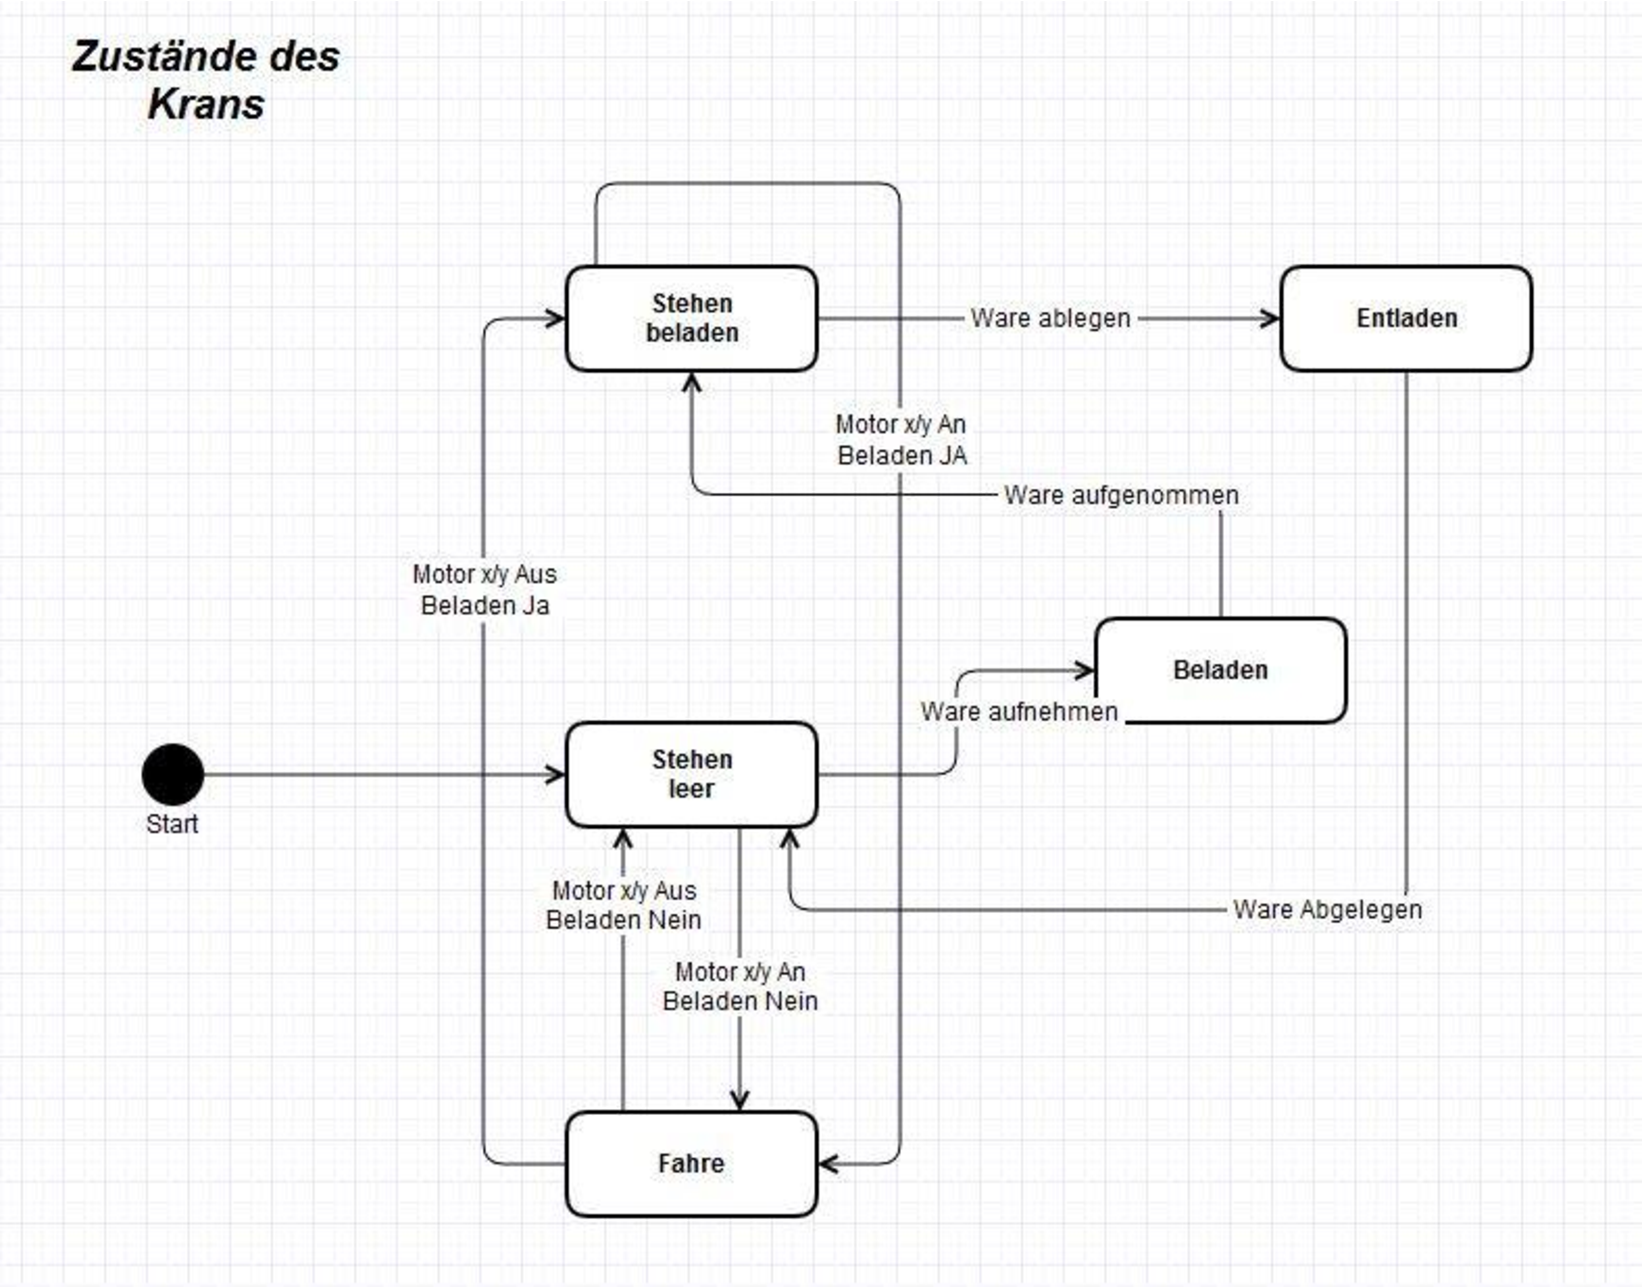
\includegraphics[scale=0.53]{Zustand.pdf}\\
\begin{small}Zustandsdiagramm des Krans\end{small}\\
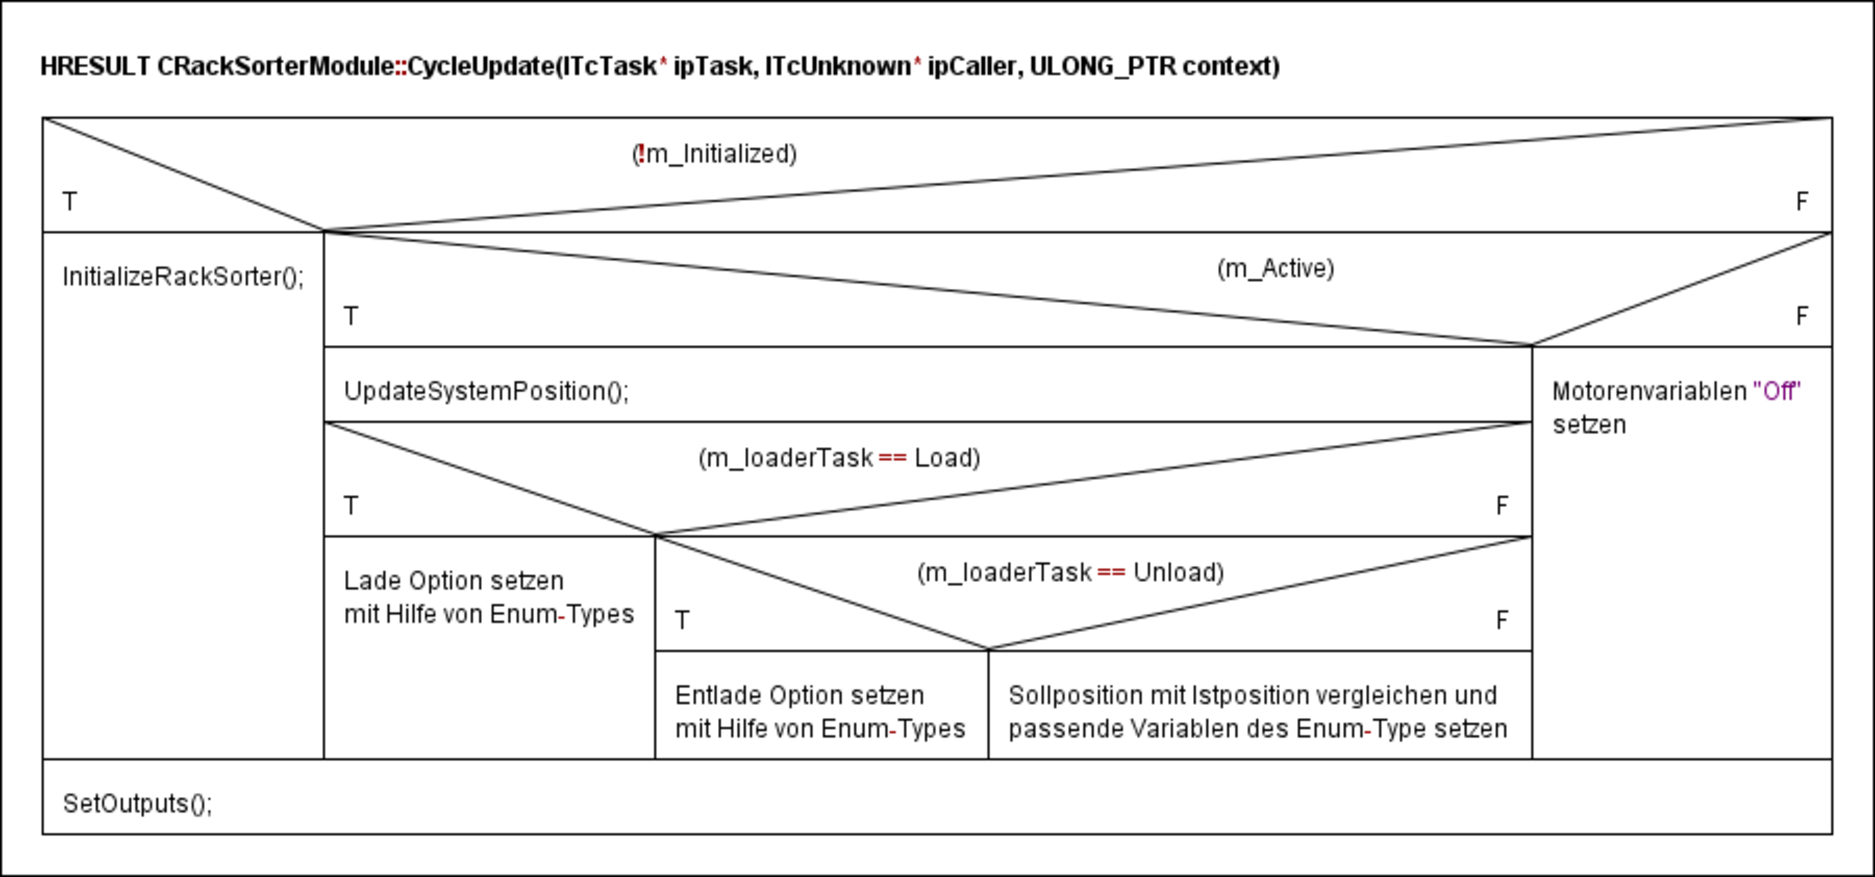
\includegraphics[scale=0.45]{HRESULT_CRackSorterModule.pdf}\\
\begin{small}Struktogramm der CycleUpdate\end{small}\\[2pt]
\end{center}
Für die Programmstruktur wurden noch einige weitere Methoden und Typen implementiert.

\subsection{Typdefinitionen}
Für übersichtlicheren Code wurden folgende \lstinline|enum|-Typen definiert, die für interne Variablen für Zustände von Ein- und Ausgangsklemmen verwendet werden:
\begin{lstlisting}
enum MotorState {
	Forward, Backward,
	Up,	Down, Left, Right,
	Off
};
enum LoaderPosition {
	Belt, Neutral, Rack
};
\end{lstlisting}

\subsection{void CRackSorterModule::InitializeRackSorter()}
Die Initialisierung-Routine prüft jede Achse auf „Neutral-Position“. Ist der Kran nicht in dieser Position oder kann die Position nicht bestimmt werden (da kein Schalter betätigt wird), werden die Achsen des Krans nacheinander in diese Vorgabe überführt. Dabei ist wichtig, zuerst sicher zu stellen, dass der Schlitten in seiner neutralen Position ist, um Schäden an Kran oder Regal zu vermeiden.
Die Methode wird nur ausgeführt, wenn die Member-Variable m\_initialized "false"\ ist und setzt diese Variable auf "true", sobald alle Achsen des Krans in der „Neutral-Position“ angekommen sind.

\subsection{void CRackSorterModule::UpdateSystemPosition()}
In jedem Takt wird mithilfe der am Hochregallager angebrachten Schalter die aktuelle Position des Krans bestimmt. Ist ein Schalter für eine Achse betätigt, befindet sich der Kran an dieser Position. Ist kein Schalter betätigt, wird für diese Achse die letzte bekannte Position beibehalten.

\subsection{void CRackSorterModule::SetOutputs()}
Die internen Ausgänge \lstinline|MotorState xMotor, yMotor, zMotor| werden hier vom \lstinline|MotorState enum|-Typen in jeweils zwei boolsche Werte für die Ausgangsklemmen der Steuerung übersetzt und die Ausgänge entsprechend geschaltet. Für \lstinline|xMotor| \zb{}:
\begin{lstlisting}[basicstyle=\ttfamily\footnotesize]
	switch (m_xMotor) {
	case Left:
		m_Outputs.x_motor_right = false;
		m_Outputs.x_motor_left = isPWM;
		break;
	case Right:
		m_Outputs.x_motor_left = false;
		m_Outputs.x_motor_right = isPWM;
		break;
	case Off:
	default:
		m_Outputs.x_motor_left = false;
		m_Outputs.x_motor_right = false;
		break;
	}
\end{lstlisting}

\newpage
\chapter{Kommunikation mit ADS}
\section{Einführung ADS}
Die Automation Device Specification (ADS) beschreibt eine Schnittstelle die es erlaubt, über Netzwerk (TCP/IP) mit einem TwinCAT-Modul zu kommunizieren. Dabei stellt das TwinCAT-Modul den Server dar. Ein ADS-Paket beginnt – nach Adresse und Port des Zielgeräts – mit einer Group- und einer Offset-ID, die gemeinsam die Adresse des ADS-Befehls beschreiben.

Die Funktion \lstinline|adsReadWrite| ermöglicht es, gleichzeitig Daten an den ADS-Server schicken und von ihm empfangen kann. So lassen sich Rückgabewerte für Funktionsaufrufe realisieren. Dieses Moduls hat zwei Gruppen mit je vier Offsets definiert.

\section{Spezifikation}
\begin{center}
\begin{tabular}{ l p{3.1cm} p{4.4cm} p{4.5cm} }
\hline
\multicolumn{4}{c}{\textbf{Group 1}} \\ \hline
\textbf{Offset} & \textbf{Funktion} & \textbf{Write Data} & \textbf{Read Data} \\ \hline
1 & System Enable / Disable & bool: True: Enable; False: Disable & bool: Always True \\ \hline
2 & Aktuelle Position & (any) & UINT16: L: y-Pos; H: x-Pos \\ \hline
3 & Ist Kran beladen? & (any) & bool: True: beladen; False: nicht beladen \\ \hline
4 & Init/Reset & bool: True: Reset; False: Abfrage Initialisiert? & bool: True wenn Reset; m\_Initialized wenn Abfrage \\ \hline \hline
\multicolumn{4}{c}{\textbf{Group 2}} \\ \hline
1 & Gehe zu Ladeposition & UINT16: L: y-Pos; H: x-Pos & UINT8 AdsResponse \\ \hline
2 & Gehe zu Entladeposition & UINT16: L: y-Pos; H: x-Pos & UINT8 AdsResponse \\ \hline
3 & Lade Element & (any) & UINT8 AdsResponse \\ \hline
4 & Entlade Element & (any) & UINT8 AdsResponse \\ \hline
\end{tabular}
\end{center}
Der Typ \lstinline|AdsResponse| ist dabei wie folgt definiert:
\begin{lstlisting}
enum AdsResponse : UINT8 {
	OK = 0x00,
	BUSY = 0x01,
	ERROR_CLIENT = 0x02,
	ERROR_SERVER = 0x04
} 
\end{lstlisting}
\lstinline|BUSY| bedeutet dabei, dass die Steuerung gerade dabei ist, eine zuvor angeforderte Bewegung auszuführen. Nur bei \lstinline|OK| wird der Befehl ausgeführt. \lstinline|ERROR_CLIENT| wird zurückgegeben, wenn die angeforderte Position außerhalb der Dimensionen des Lagers liegt oder wenn ein Lade-Befehl geschickt wird, wenn das Lager an einer Entlade-Position steht (und umgekehrt). \lstinline|ERROR_SERVER| ist definiert, aber ungenutzt.

Wenn "(any)"\ in der ADS-Tabelle steht, verlangt die entsprechende Funktion keine Parameter. Da alle Funktionen innerhalb des \lstinline|adsReadWrite|-Kontext implementiert sind, erfordert der Aufruf ein Byte Nutzdaten, die aber nicht gelesen werden.

\section{pyads}
Das Paket und Modul \pyads\ [4] stellt einen Python-Wrapper für die unter MIT-Lizenz veröffentlichte ADS-Bibliothek [5] bereit. Es lässt sich einfach aus dem Python Package Index installieren:
\begin{lstlisting}
pip install pyads
\end{lstlisting}
Es bietet einen vollwertigen Zugriff auf die ADS-Schnittstelle. Ein \lstinline|adsReadWrite|-Aufruf um das Hochrregallager zu aktivieren (Group 1, Offset 1), sähe zum Beispiel, inklusive erstellen und öffnen der Verbindung zum lokalen TwinCAT-Modul, so aus:
\begin{lstlisting}
plc = pyads.Connection('127.0.0.1.1.1', pyads.PORT_SPS1)
plc.open()
plc.read_write(1, 1, pyads.PLCTYPE_BOOL, True, pyads.PLCTYPE_BOOL)
\end{lstlisting}

Da Python keine strikten Typen besitzt, müssen diese bei Zugriff auf eine C-API angegeben werden. Der letzte Parameter gibt an, welcher Datentyp vom ADS-Server gelesen werden soll. Die gelesenen Daten werden von der Funktion zurückgegeben.

\newpage
\chapter{GUI mit Qt}
Um die Bedienung von \racksorter\ im Zusammenspiel mit \pyads\ zu erleichtern, wurde eine kleine grafische Benutzeroberfläche in Qt entworfen.
\begin{center}
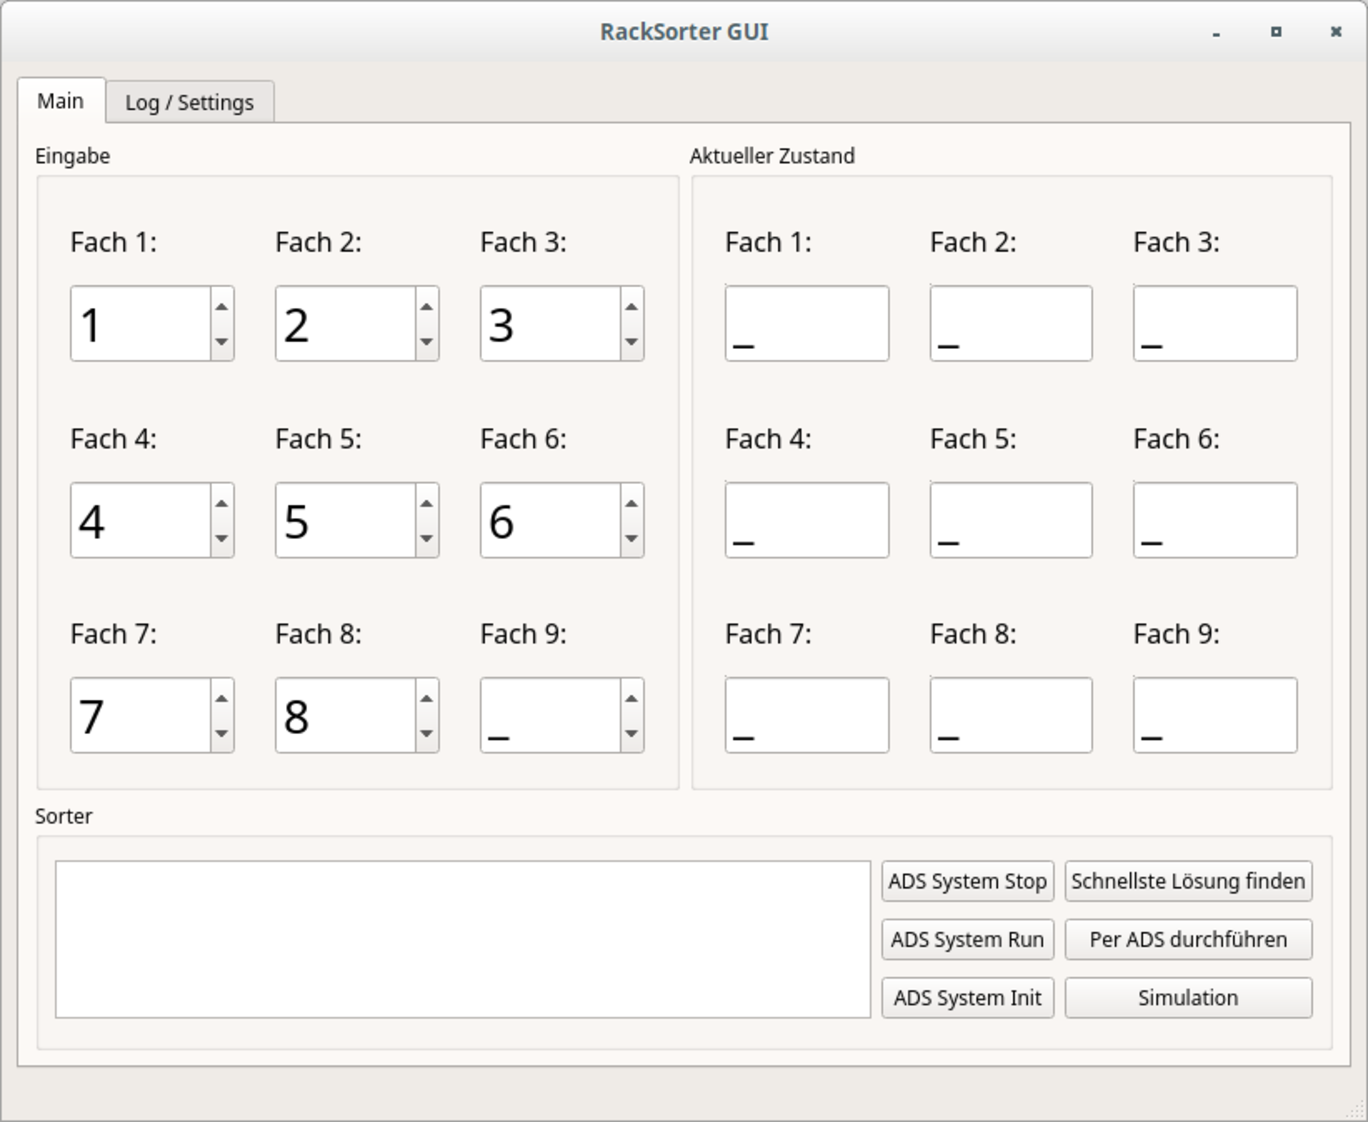
\includegraphics[scale=0.4]{GUI1.pdf}
\end{center}
Auf der linken Seite lässt sich eine Permutation des Hochrregallagers einstellen. Man kann mit Klick auf den entsprechenden Button mit Hilfe des \racksorter-Moduls die schnellste Lösung finden. Außerdem lassen sich die Lösung per ADS mit dem Hochregallager-Modell durchführen und eine Simulation innerhalb der GUI darstellen.
\begin{center}
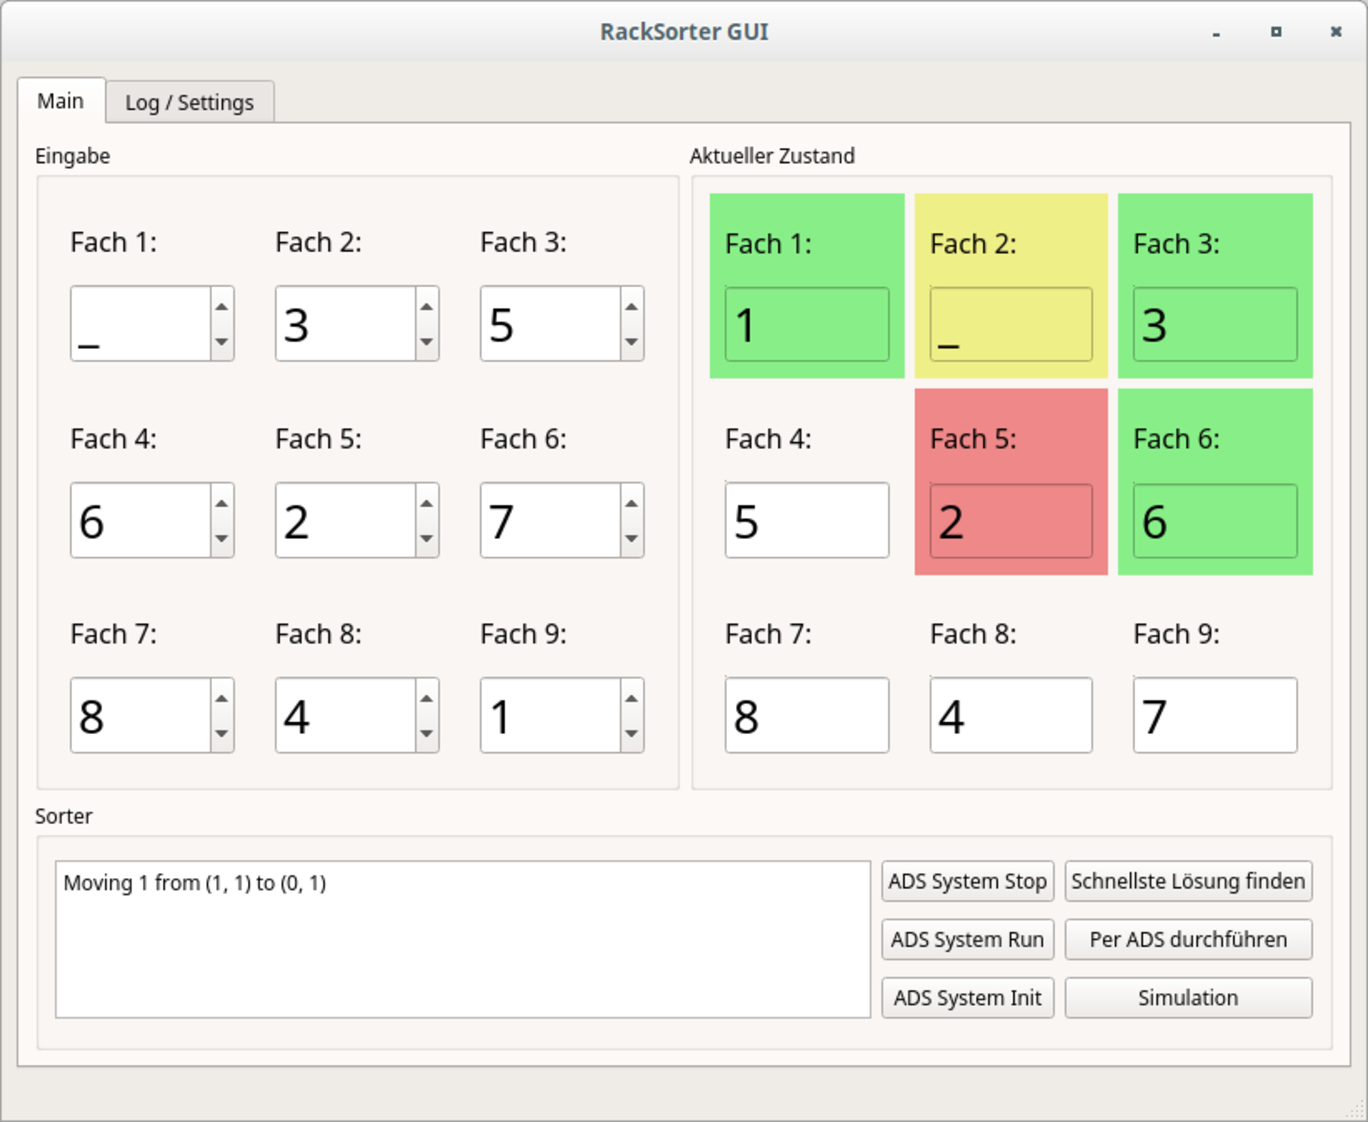
\includegraphics[scale=0.4]{GUI3.pdf}
\end{center}
\begin{center}
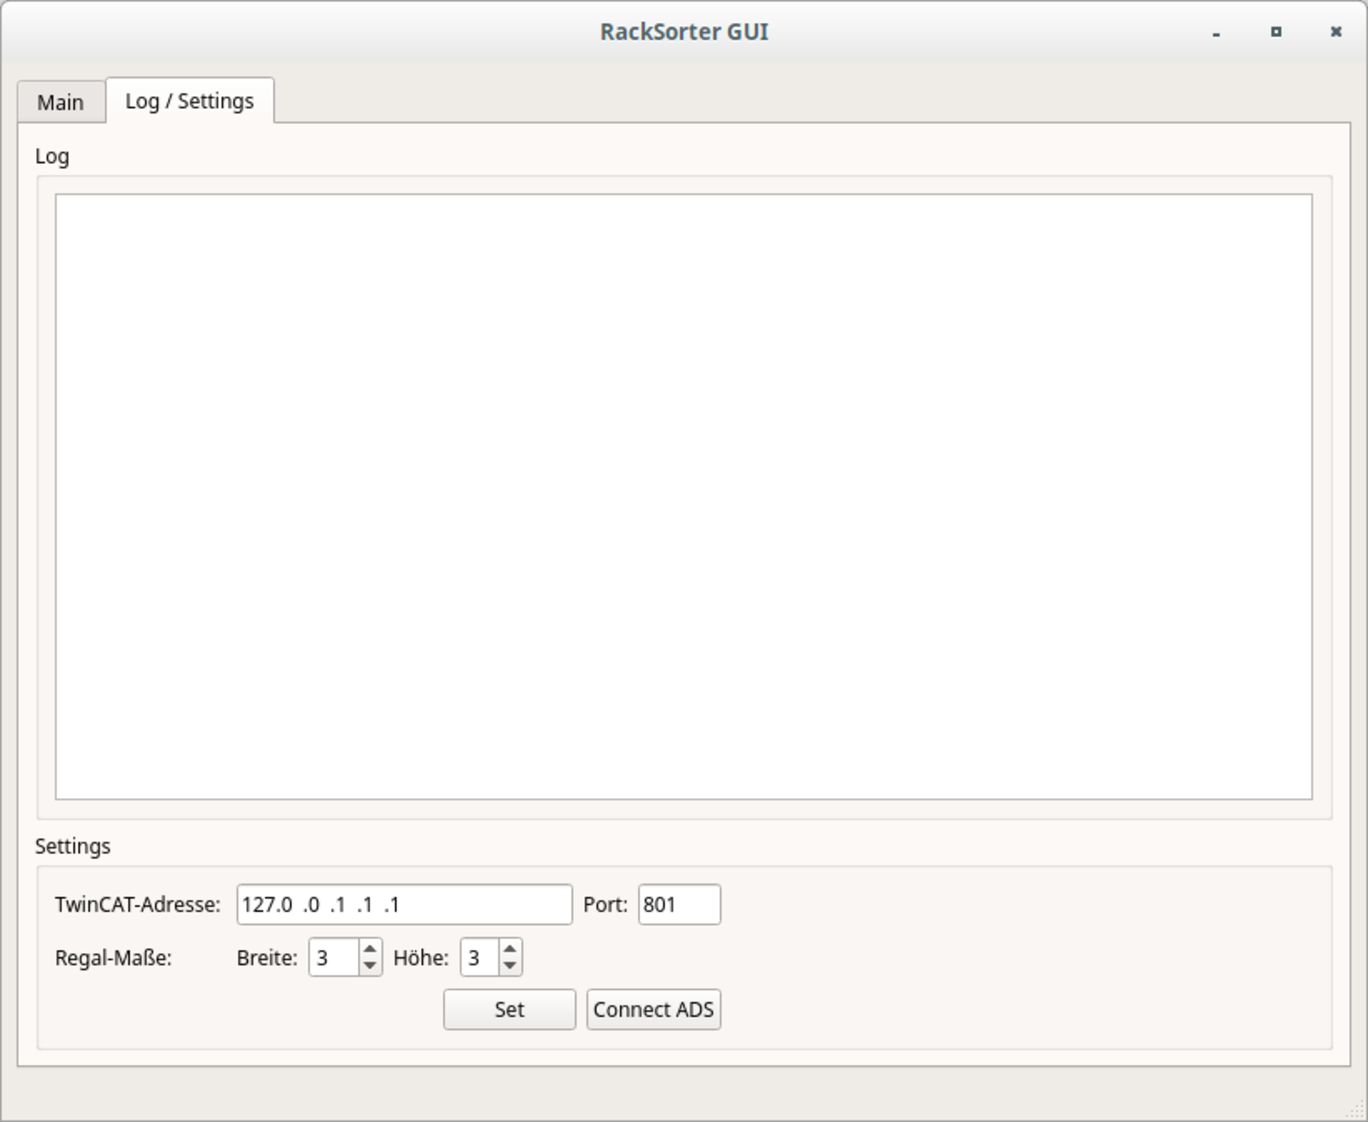
\includegraphics[scale=0.4]{GUI2.pdf}
\end{center}
Im Tab "Log/Settings" besteht die Möglichkeit, Adresse und Port für die ADS-Verbindung einzustellen sowie die Dimensionen des Hochregallagers, mit dem gearbeitet werden soll. Diese Einstellung ist auf die realen Dimensionen von $4 x 10$ beschränkt.

Die Ein- und Ausgabefelder im "Main"-Tab werden bei einem Klick auf "Set" entsprechend angepasst:
\begin{center}
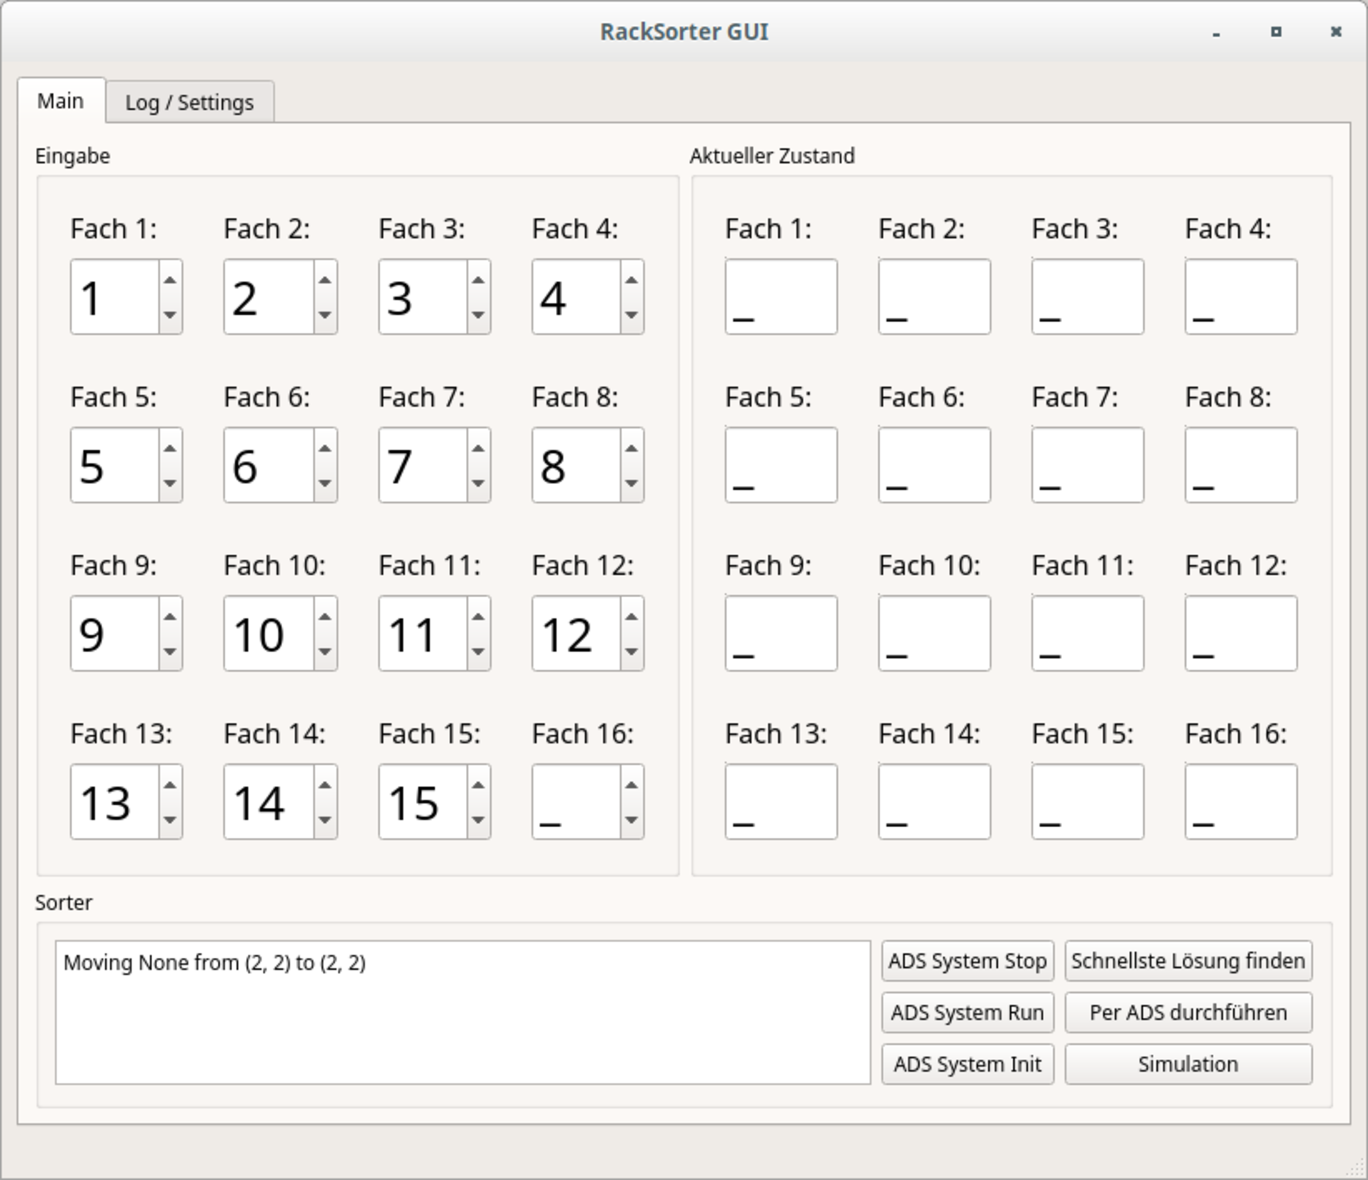
\includegraphics[scale=0.4]{GUI4.pdf}
\end{center}

\newpage
\chapter{Zusammenfassung}
Die gesetzten Ziele konnten umgesetzt werden, eine Clientsoftware errechnet durch rekursives Verhalten den kürzesten Weg um das Hochregallager zu sortieren und gibt jeden Schritt an das Runtime-Modul weiter. Als Schritt wird das Be-/Entladen oder Fahre nach x/y beschrieben. Ein GUI wurde Programmiert welche es dem Benutzer ermögliche das System zu starten, das Hochregallager zu definieren, sowie die einzelnen Schritte zu verfolgen. Das TwinCAT-Modul wurde in der Sprache C++ umgesetzt und die Berechnung des Weges sowie die GUI wurden in Python entwickelt.

Das Modul ist so programmiert, dass sie möglichst einfach weiterentwickelt werden kann. So können z.B. weitere ADS Groups und Offsets dazu programmiert werden (s. Kapitel 4). Auch weitere Sortieralgorithmen können, sollten sie an die vorhandenen ADS Groups angepasst, in kürzester Zeit implementiert werden, da hier, vereinfacht beschrieben mit „Fahre nach“ oder „Belade“ gearbeitet wird.

Die Ziele wurden zwar erfüllt, allerdings könnte das Projekt noch weiter angepasst werden, z.B. an die aktuellen Gegebenheiten wie Smartphones und Cloudcomputing. Jedoch muss dazu gesagt werden, dass wir feststellen mussten, dass die Zeit, die zur Berechnung des kürzesten Weges mit Wachstum der Anlage in Dimensionen wächst, welche nicht Wirtschaftlich sind.

\backmatter
\chapter{Quellen und weiterführende Links}
\begin{tabular}{l l}
{[1]} & Permutation of a set. In Encylopaedia of Mathematics \\
	& \textit{https://www.encyclopediaofmath.org/index.php/Permutation\_of\_a\_set} \\
{[2]} & TwinCAT C++ Dokumentation \\
	& \textit{http://download.beckhoff.com/download/document/automation/twincat3/}\\
	& \textit{TC1300\_C\_DE.pdf} \\
{[3]} & Beckhoff Information System: Einführung ADS \\
	& \textit{https://infosys.beckhoff.de/index.php?content=../content/1031/}\\
	& \textit{TcAdsCommon/HTML/TcAdsCommon\_IntroAds.htm} \\
{[4]} & pyads \\
	& \textit{https://github.com/stlehmann/pyads} \\
{[5]} & Beckhoff ADS Library \\
	& \textit{https://github.com/Beckhoff/ADS} \\
  {[S1]} & RackSorterPython \\
  & \textit{https://github.com/WolleTD/RackSorterPython} \\
  {[S2]} & RackSorter Runtime \\
  & \textit{https://github.com/WolleTD/RackSorter} \\
\end{tabular}
\newpage
\end{document}